% Created 2017-06-02 Fri 14:52
\documentclass[presentation]{beamer}
\usepackage[utf8]{inputenc}
\usepackage[T1]{fontenc}
\usepackage{fixltx2e}
\usepackage{graphicx}
\usepackage{longtable}
\usepackage{float}
\usepackage{wrapfig}
\usepackage{rotating}
\usepackage[normalem]{ulem}
\usepackage{amsmath}
\usepackage{textcomp}
\usepackage{marvosym}
\usepackage{wasysym}
\usepackage{amssymb}
\usepackage{hyperref}
\tolerance=1000
\usepackage{tabu}
\usepackage{minted}
\usepackage[english, ngerman]{babel}
\hypersetup{pdfauthor="Vasilij Schneidermann", pdftitle="Interim - Zwischen Plan 9 und Lisp Machine", colorlinks, linkcolor=black, urlcolor=blue}
\uselanguage{German}
\languagepath{German}
\usetheme{Rochester}
\usecolortheme[RGB={87,83,170}]{structure}
\author{Vasilij Schneidermann}
\date{Juni 2017}
\title{Interim - Zwischen Plan 9 und Lisp Machine}
\hypersetup{
  pdfkeywords={},
  pdfsubject={},
  pdfcreator={Emacs 25.2.1 (Org mode 8.2.10)}}
\begin{document}

\maketitle
\begin{frame}{Outline}
\tableofcontents
\end{frame}

\AtBeginSection{\frame{\sectionpage}}
\shorthandoff{"}

\section{Einführung}
\label{sec-1}

\begin{frame}[label=sec-1-1]{Sprecher}
\begin{itemize}
\item Vasilij Schneidermann, 24
\item Wirtschaftsinformatikstudent
\item Software-Entwickler bei \href{https://www.bevuta.com/en/}{bevuta IT GmbH}
\item mail@vasilij.de
\item \url{https://github.com/wasamasa}
\item \url{http://emacshorrors.com/}
\item \url{http://emacsninja.com/}
\end{itemize}
\end{frame}

\begin{frame}[label=sec-1-2]{Grundlegendes Problem}
\begin{itemize}
\item Moderne Computer sind komplex
\item Unmöglich den gesamten Stack zu verstehen
\item Walled Gardens breit akzeptiert
\item Kontrollverlust über das Betriebssystem
\item Wird es jemals besser?
\end{itemize}
\end{frame}

\begin{frame}[label=sec-1-3]{Damals war alles besser™}
\begin{figure}[htb]
\centering
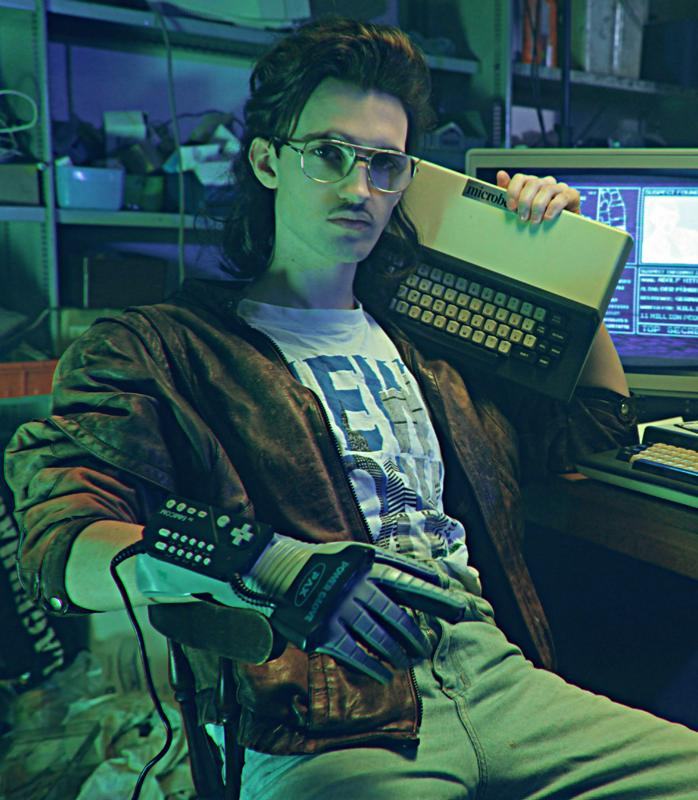
\includegraphics[height=6cm]{./images/hackerman.jpg}
\caption{Hackerman (Kung Fury)}
\end{figure}
\end{frame}

\begin{frame}[label=sec-1-4]{Damals war alles \sout{besser™} einfacher}
\begin{itemize}
\item Bestseller: Commodore 64 (1982)
\item Boot in einen BASIC-Prompt
\item Umfangreiches Handbuch für Reparaturen
\item Populär in der Demoszene
\item Verwendet für BBS
\item Später durch den Amiga verdrängt
\end{itemize}
\end{frame}

\begin{frame}[label=sec-1-5]{Wie würde ein moderner C64 aussehen?}
\begin{itemize}
\item RISC-Prozessor
\item High-Level Programmiersprache
\item Benutzeranpassbares Betriebssystem
\item 1920x1080 ansteuerbare Pixel in 16-/24-Bit Farbe
\item Keyboard und mausgesteuerte Benutzereingabe
\item Audio-Output in CD-Qualität
\item Netzwerkanbindung über Ethernet
\end{itemize}
\end{frame}

\begin{frame}[label=sec-1-6]{Wie würde ein einfacheres Betriebssystem aussehen?}
\begin{itemize}
\item Plan 9
\item Lisp Machine
\item Project Oberon
\end{itemize}
\end{frame}

\begin{frame}[label=sec-1-7]{Motivation für diesen Vortrag}
\begin{itemize}
\item \href{https://www.arrdem.com/2014/11/28/the_future_of_the_lispm/}{The Future of the LispM}
\item Beschreibung einer Alternative zur Lisp Machine:
\begin{itemize}
\item Betriebssystem mit JIT-Compiler
\item Moderne Lisp-Implementierung
\item Plan 9 statt Unix
\end{itemize}
\item \href{http://dump.mntmn.com/interim-paper/}{Interim} erfüllt diese Kriterien und mehr
\end{itemize}
\end{frame}

\section{Interim - Aufbau}
\label{sec-2}

\begin{frame}[label=sec-2-1]{Vorab}
\begin{itemize}
\item Sämtliche Aussagen über Interim beziehen sich auf meinen Fork auf
\url{https://github.com/wasamasa/interim/tree/next}
\item Enthält zusätzliche Dokumentation, Bugfixes und Features
\end{itemize}
\end{frame}

\begin{frame}[label=sec-2-2]{Betriebsmodi}
\begin{itemize}
\item Typischerweise OS für eine Zielplattform entwickelt
\item Testen im Emulator oder auf echter Hardware
\item Interim unterstützt \emph{Hosted Mode} und \emph{Bare Metal}
\end{itemize}
\end{frame}

\begin{frame}[fragile,label=sec-2-3]{Hosted Mode}
 \begin{itemize}
\item Lisp-Interpreter als Kern
\item Kann auf POSIX-kompatiblem System mit \texttt{libc} ausgeführt werden
\item Nutzt SDL2 für Maus, Tastatur und Framebuffer
\item Läuft auf Linux, Windows, OS X
\item Experimenteller Support für AmigaOS
\end{itemize}
\end{frame}

\begin{frame}[fragile,label=sec-2-4]{Bare Metal}
 \begin{itemize}
\item Portierung des Interpreters auf System ohne \texttt{libc}
\item Verwendung von \href{https://sourceware.org/newlib/}{newlib} als \texttt{libc}
\item Assembler für Setup des \emph{Stacks} und Boot ins Programm nötig
\item Systemspezifische Geräteabstraktionen
\item Läuft auf Raspberry Pi 2
\item Experimenteller Support für regulären x86-PC
\end{itemize}
\end{frame}

\begin{frame}[label=sec-2-5]{Boot (Hosted Mode)}
\begin{itemize}
\item Init des JIT-Compilers
\item Init von Dateisystemen
\item Einlesen einer Datei
\item Alternativ: Start der REPL
\end{itemize}
\end{frame}

\begin{frame}[label=sec-2-6]{Boot (Bare Metal)}
\begin{itemize}
\item BSS-Sektion initialisieren
\item Stack-Setup
\item Start des Kernels
\item Hardware-Setup (MMU, UART, Framebuffer, USB, \ldots{})
\item Init des JIT-Compilers
\item Init von Dateisystemen
\item Start der grafischen REPL
\end{itemize}
\end{frame}

\begin{frame}[fragile,label=sec-2-7]{Device-Abstraktion}
 \begin{itemize}
\item Idee: Gleiche API für ähnliche Hardware
\item Implementierungen können grundverschieden sein
\item Erlaubt Entwicklung in Hosted Mode und Testen auf Bare Metal
\item Beispiel: Keyboard in \texttt{/devices/sdl2.c}, \texttt{/devices/rpi2/uartkeys.c}
  und \texttt{/devices/rpi2/usbkeys.c} implementiert
\end{itemize}
\end{frame}

\begin{frame}[label=sec-2-8]{Compiler}
\begin{itemize}
\item Problem: Naiver Interpreter zu langsam, AOT-Compiler nicht anwendbar
\item Lösung: Inkrementeller JIT-Compiler (vgl. Tracing JIT-Compiler)
\item Abstraktion von ISA-spezifischen Instruktionen (x86, amd64, m68k, arm64)
\item Kompilieren von Lisp zu diesem Instruktions-Set
\item Schreiben des Codes in ausführbaren Speicher
\item Cast zu Funktionspointer und Aufruf
\item Probleme: Calling Convention, Memory Barriers, Debugging schwierig
\end{itemize}
\end{frame}

\begin{frame}[label=sec-2-9]{"Multitasking"}
\begin{itemize}
\item Single-tasked
\item Emulation von kooperativem Multi-Tasking
\item Liste von Tasks (Funktionen)
\item Wiederholte Iteration über Taskliste
\end{itemize}
\end{frame}

\section{Interim - Sprache}
\label{sec-3}

\begin{frame}[label=sec-3-1]{Grundeigenschaften}
\begin{itemize}
\item Es ist ein Lisp!
\item Homoikonisch, minimalistisch, high-level
\item Features: Globale/lokale Variablen, Integer-Arithmetik, einfache
Kontrollstrukturen, Listen/Array-Manipulation, Introspektion,
Dateisystemzugriff
\item Typen: Integers, Strings, Byte-Arrays, Funktionen, Listen, Structs
\item Manuelle Garbage Collection
\end{itemize}
\end{frame}

\begin{frame}[fragile,label=sec-3-2]{Unterschiede zu anderen Lisp-Dialekten}
 \begin{itemize}
\item \texttt{let} ohne Body, nur in Funktionen zulässig
\item \texttt{do} ist nie implizit
\item Keine Makros oder Fexprs
\item Kein syntaktischer Zucker (Readermakros)
\item Keine Booleans (siehe C!)
\item Serialisierung nur mit fixen Buffern möglich (kein \texttt{str})
\item Minimale Standardbibliothek (beinhaltet \texttt{or}, \texttt{strlen}, \texttt{sin}, \ldots{})
\end{itemize}
\end{frame}

\begin{frame}[fragile,label=sec-3-3]{Beispiele}
 \begin{minted}[]{lisp}
(def greeting "Hello World!")
(print greeting) ;=> "Hello World!"

(put8 greeting 11 (get8 "?" 0))
(print greeting) ;=> "Hello World?"
\end{minted}
\end{frame}

\begin{frame}[fragile,label=sec-3-4]{Beispiele}
 \begin{minted}[]{lisp}
(+ 1 1) ;=> 2
(cons 1 2) ;=> (1 . 2)
(list 1 2) ;=> (1 2)
(cons 1 (cons 2 nil)) ;=> (1 2)

(def bytes [1234])
(put8 bytes 0 0x34)
(put8 bytes 1 0x12)
bytes ;=> [3412]
\end{minted}
\end{frame}

\begin{frame}[fragile,label=sec-3-5]{Beispiele}
 \begin{minted}[]{lisp}
(def factorial
 (fn n
  (do
   (let i 1)
   (let result 1)
   (while (lt i n)
    (do
     (let i (+ i 1))
     (let result (* result i))))
   result)))

(factorial 4) ;=> 24
\end{minted}
\end{frame}

\section{Interim - Dateisysteme}
\label{sec-4}

\begin{frame}[fragile,label=sec-4-1]{Plan 9-Dateisysteme}
 \begin{itemize}
\item Jedes Gerät wird unter einem Pfad gemountet
\item Mounten erforder folgende Handler:
\begin{itemize}
\item \texttt{open}: Öffnen eines Stream-Objekts für den gegebenen Pfad
\item \texttt{mmap}: Anfordern einer alternativen Repräsentation des Pfads
\item \texttt{recv}: Auslesen eines Objekts aus dem gegebenen Stream
\item \texttt{send}: Schreiben eines Objekts in den gegebenen Stream
\end{itemize}
\end{itemize}
\end{frame}

\begin{frame}[fragile,label=sec-4-2]{Beispiel: \texttt{/framebuffer}}
 \begin{itemize}
\item Implementierung: \texttt{/devices/sdl2.c}, \texttt{/devices/fbfs.c},
\texttt{/devices/dev\_linuxfb.c}
\item \texttt{open}: Öffnen eines Kontrollkanals für den \emph{Framebuffer}
\item \texttt{mmap}: Anfordern des \emph{Framebuffers} in Form eines Byte-Arrays
\item \texttt{recv}: Gibt Liste von Attributen oder Attribute selbst aus
\item \texttt{send}: Löst eine \emph{Blit}-Operation aus
\end{itemize}
\end{frame}

\begin{frame}[fragile,label=sec-4-3]{Beispiel: Framebuffer-Parameter}
 \begin{minted}[]{lisp}
(def fb (open "/framebuffer"))
(def refresh (fn (send fb 0)))
(def load (fn path (recv (open path))))

(def width (load "/framebuffer/width"))
(def height (load "/framebuffer/height"))
(def depth (load "/framebuffer/depth"))

(def pitch (* width depth))
(print (* height pitch)) ;=> 960000
\end{minted}
\end{frame}

\begin{frame}[fragile,label=sec-4-4]{Beispiel: Framebuffer-Manipulation}
 \begin{minted}[]{lisp}
(def pixels (mmap "/framebuffer"))
(def black 0x0000)

(def paint-pixel
 (fn x y color
  (do
   (let offset (+ (* y pitch) (* x depth)))
   (put16 pixels offset color))))

(paint-pixel 0 0 black)
\end{minted}
\end{frame}

\begin{frame}[fragile,label=sec-4-5]{Beispiel: \texttt{sledge/demos/palette.l}}
 \begin{itemize}
\item Idee: Framebuffer erlaubt $2^{8*bpp}$ Farben
\item Bei 2bpp: Farbwerte zwischen $0$ und $65535$
\item Quadrat mit jedem Farbwert: Palette
\end{itemize}
\end{frame}

\begin{frame}[fragile,label=sec-4-6]{Beispiel: \texttt{/sd}}
 \begin{itemize}
\item Implementierung: \texttt{/devices/posixfs.c}, \texttt{/devices/fatfs.c}
\item \texttt{open}: Nicht implementiert
\item \texttt{mmap}: Nicht implementiert
\item \texttt{recv}: Gibt Liste von Verzeichniseinträgen oder Dateinhalt zurück
\item \texttt{send}: Schreibt in eine Datei
\end{itemize}
\end{frame}

\begin{frame}[fragile,label=sec-4-7]{Beispiel: Laden eines Bilds}
 Vorbereitung:

\begin{minted}[]{bash}
ffmpeg -i image.jpg -vcodec rawvideo -f rawvideo\
  -pix_fmt rgb565 image.565
\end{minted}

Laden:

\begin{minted}[]{lisp}
(def load (fn path (recv (open path))))
(def image (load "/sd/image.565"))
\end{minted}
\end{frame}

\begin{frame}[fragile,label=sec-4-8]{Beispiel: \texttt{sledge/demos/grumpycat.l}}
 \begin{itemize}
\item Kenntnis von Breite und Höhe nötig
\item \emph{Image Loader} ist nicht nötig
\item Jeder Bildpixel wird an die richtige Stelle positioniert
\end{itemize}
\end{frame}

\begin{frame}[fragile,label=sec-4-9]{Beispiel: \texttt{sledge/demos/helloworld.l}}
 \begin{itemize}
\item Fontformate sind sehr komplex
\item Alternative: Speichern von GNU Unifont als Bitmap
\item Position jedes Zeichens ist errechenbar
\item Kopieren von Zeichen auf richtige Position am Framebuffer
\item Sogar Cursor so implementierbar!
\end{itemize}
\end{frame}

\begin{frame}[fragile,label=sec-4-10]{Beispiel: \texttt{sledge/demos/screenshot.l}}
 \begin{itemize}
\item Roher Screenshot ist trivial
\item Screenshot zu Format tricky wegen Kompression, Pixelformaten
\item BMP und TGA sind die einfachsten Formate, aber:
\begin{itemize}
\item TGA unterstützt kein kompatibles Pixelformat
\item BMP ist unterspezifiziert, wird je nach Viewer verschieden
angezeigt
\end{itemize}
\end{itemize}
\end{frame}

\begin{frame}[fragile,label=sec-4-11]{Beispiel: \texttt{sledge/demos/munchingsquares.l}}
 \begin{itemize}
\item Klassische Demo von 1962
\item Animation besteht aus Zeichnen aller Pixel und Warten
\item Warten durch Ausführen von \texttt{(gc)} implementiert
\item Algorithmus: Für Frame $n$ zwischen 1 und 16:
\begin{itemize}
\item $x$ xor $y < n$
\item Wenn wahr, ist der Pixel schwarz, sonst weiß
\end{itemize}
\end{itemize}
\end{frame}

\begin{frame}[fragile,label=sec-4-12]{Beispiel: \texttt{/keyboard}}
 \begin{itemize}
\item Implementierung: \texttt{/devices/sdl2.c}, \texttt{/devices/rpi2/uartkeys.c},
\texttt{/devices/rpi2/usbkeys.c}
\item \texttt{open}: Nicht implementiert
\item \texttt{mmap}: Nicht implementiert
\item \texttt{recv}: Gibt aktuell gedrückte Taste oder \texttt{nil} zurück
\item \texttt{send}: Nicht implementiert
\end{itemize}
\end{frame}

\begin{frame}[fragile,label=sec-4-13]{Beispiel: \texttt{sledge/demos/bounce.l}}
 \begin{itemize}
\item Zeichnen eines Quadrats an einer Position
\item Übermalen des Quadrats an alter Position in weiß
\item Errechnen einer neuen Position
\item Ändern der Richtung bei Erreichen der Kante
\item Bonus: Drücken von Tasten ändert die Farbe
\end{itemize}
\end{frame}

\begin{frame}[fragile,label=sec-4-14]{Weitere nicht abgedeckten APIs}
 \begin{itemize}
\item Maus (\texttt{/mouse})
\item Netzwerk (\texttt{/net})
\item Implementierung eigener Dateisysteme aus Lisp heraus
\end{itemize}
\end{frame}

\section{Weitere Schritte}
\label{sec-5}

\begin{frame}[label=sec-5-1]{Verbessern der Sprache}
\begin{itemize}
\item First-class functions
\item Makros und Readermakros
\item Automatische \emph{Garbage Collection}
\item Mehr Datentypen (Vector, Hash Map)
\item Prädikate, mehr Introspektion
\item Exceptions
\end{itemize}
\end{frame}

\begin{frame}[fragile,label=sec-5-2]{Komfortfeatures}
 \begin{itemize}
\item Mehr Fehler signalisieren
\item Optionale Argumente / Varargs / \texttt{apply}
\item Escapes in Strings
\item Besserer Printer und Print-Funktionen
\item Debugging-Funktionalität
\item Ersetzen von \texttt{fn} / \texttt{while} durch Makro mit \texttt{do}
\end{itemize}
\end{frame}

\begin{frame}[label=sec-5-3]{Testsuite für Sprachfeatures}
\begin{itemize}
\item Die aktuelle Dokumentation ist nicht auf dem neuesten Stand
\item Viele Demonstrationsprogramme welche nicht mehr funktionieren
\item Einige Features sind kaputt (teilweise nur auf einer Plattform)
\item Integration von CI
\end{itemize}
\end{frame}

\begin{frame}[fragile,label=sec-5-4]{APIs}
 \begin{itemize}
\item Verhalten in \emph{Hosted Mode} an \emph{Bare Metal} anpassen
\item Implementierung der \texttt{delete}-Operation
\item Implementierung weiterer APIs:
\begin{itemize}
\item \texttt{/arch}, \texttt{/sys} (Systeminformationen)
\item \texttt{/time} (kein \texttt{sleep} bisher möglich)
\end{itemize}
\end{itemize}
\end{frame}

\begin{frame}[fragile,label=sec-5-5]{Verbessern der Demos}
 \begin{itemize}
\item Spiele (\texttt{mario.l}, \texttt{gtn.l})
\item Grafische Shell und Editor (\texttt{shell.l}, \texttt{editor.l})
\item Netzwerk (HTTP, IRC)
\end{itemize}
\end{frame}

\begin{frame}[fragile,label=sec-5-6]{Bugs beheben}
 Kleine Auswahl:
\begin{itemize}
\item GC rührt lokale Variablen an
\item \emph{Undefined Behavior}
\item Segfault bei Verwendung von \texttt{put32}
\item Off-by-one in String-Funktionen
\item Minimum an Fehlerbehandlung
\end{itemize}
\end{frame}

\begin{frame}[label=sec-5-7]{Bauen eines besseren Interim}
\begin{itemize}
\item Vielleicht ist die einfachste Lösung von neuem anzufangen\ldots{}
\item Ermöglicht neue Design-Entscheidungen:
\begin{itemize}
\item Byte-Code Interpreter statt JIT-Compiler
\item Wiederverwendung von Libraries (Ragel, QBE, \ldots{})
\item Bessere Lisp-Implementierung
\item Alternative zu C
\end{itemize}
\end{itemize}
\end{frame}

\begin{frame}[label=sec-5-8]{Fragen?}
\end{frame}
% Emacs 25.2.1 (Org mode 8.2.10)
\end{document}